\BiChapter{受限玻尔兹曼机}{RBM}\label{chapter:RBM}
统计学习并不在乎事物的本质是什么,我们更关心的是数据的分布是怎样的,为了描述数据的分布,我们往往引入各种各样的模型刻画这种分布,比如,贝叶斯决策论中我们引入多维高斯分布,支持向量机中我们引入最大间隔分离面等。对于同一个任务,采用不同的模型得到的结果是不一样的,机器学习与模式识别的一个不同点在于,机器学习更注重统计,模式识别更注重于模型。例如,对于同一个任务,机器学习学者可能会假设出多个模型,再根据模型选择理论选取一个最优的模型,而模式识别学者更倾向于先大致分析这个任务更适合使用哪个模型,选取后仔细优化这个模型。尽管两者有一定的差异性,但很多方面两者是共通的,比如神经网络。神经网络并不依赖于具体的任务,也就是说,语音识别可以用神经网络处理,图像识别也可以用神经网络处理,之所以能这样做的一个原因是,神经网络的内部对于我们而言是透明的,如果我们只看重结果,希望有一个模型可以在给定一个输出的时候输出一个决策结果,不需要关心这个结果是怎么得到的,那么神经网络是一个很好的选择。神经网络的种类众多,一个分支是玻尔兹曼机,这种网络灵感源自统计物理中的玻尔兹曼分布与伊辛模型,随后,在这种网络的基础上又发展出一套受限玻尔兹曼机,通过这些网络,都可以建立数据的概率分布描述。
\BiSection{伊辛模型}
x伊辛模型是统计物理中描述物质相变的一种模型\citeup{information},是一个相互磁耦合的自旋阵列。比如在铁这种物质中,当温度降到某个程度,微观原子的自旋会表现出一定的倾向性,从而在宏观上产生磁矩,而当温度升高到一定程度时,其自旋就变得随机。

假设某个伊辛模型中有$N$个自旋的原子,对于每个原子,其状态只能取$+1$或$-1$,我们用向量$s$来表示所有原子的状态,亦即$s$代表这个伊辛模型的状态,那么我们定义该伊辛模型处于状态$s$下的能量函数为\citeup{information}
\begin{equation}
E(s; W, H) = -~\Big[\frac{1}{2} \sum\limits_{i, j = 1}^{N} w_{ij}s_is_j + \sum\limits_j Hs_j\Big]
\end{equation}

式中, $w_{ij}$代表原子$i$和原子$j$之间的耦合,如果$i$和$j$是相邻的,那么$w_{ij} = C$,否则$w_{ij} = 0$,如果常数$C>0$,那么这个模型是铁磁性的,否则是反铁磁性的。常数$H$代表作用场,$E(s; w, H)$代表能量函数,对于一般化的能量函数,我们也称之为Lyapunov函数。如果将这个能量函数推广到$H$和$W$不是常数的情况,即\citeup{information}

\begin{equation}\label{eq:energyFunction}
E(s; W, H) = -~\Big[\frac{1}{2} \sum\limits_{i, j = 1}^{N} w_{ij}s_is_j + \sum\limits_j h_js_j\Big]
\end{equation}
此时我们将得到一个物理学家称之为“自旋玻璃”的模型,这也是神经网络中的“Hopfield网络”。

\BiSection{玻尔兹曼机}
x在统计物理中,对于一个具有一定自由度的物理系统,其系统的状态是具有随机性的而不是固定的(比如房间中的氧气分子分布),假设系统处于某个状态$i$的概率为$p_i$,那么当系统与外界达到热平衡时,其概率分布为
\begin{equation}\label{zhengzefenbu}
p_i = \frac{1}{Z_T} e^{-E_i / T}
\end{equation}
式中,$T$代表系统所处的温度,$E_i$代表系统处在$i$状态下的能量,$Z_T$是在$T$温度下为了使得概率满足柯尔莫果洛夫第二公理的归一化常数。这个分布也称之为正则分布或吉布斯分布。

在机器学习中,我们往往自定义一个能量函数,然后通过正则分布建立模型,通过这种基于能量的模型来对数据进行分析。所以正则分布可以看做是机器学习与统计物理间的桥梁。

如果将式\eqref{eq:energyFunction}中的作用场去掉,并改写成矩阵形式,则得到玻尔兹曼机中的能量函数
\begin{equation}
E(s; W) = -~\frac{1}{2} s^TWs
\end{equation}

事实上,在机器学习中我们并不关心常数$T$,则玻尔兹曼分布为
\begin{equation}
p_i = \frac{1}{Z} e^{-E_i}= \frac{1}{Z} \exp\Big[\frac{1}{2} s^TWs\Big]
\end{equation}

对于一个数据对象,假设我们能观察到$n$维特征,但不仅仅代表这个数据只含$n$维特征,因此我们往往引入隐含特征的概念,假设对于一个对象,我们能观察到$v$个特征,那么我们用$v$个节点来表示这些特征,又假设我们自定义隐含的特征为$h$个,那么我们用$h$个节点来代表这个特征。比如图\ref{img:BM} 代表了含有4个可见节点和2个隐含节点的玻尔兹曼网络。
\begin{figure}[htbp]
\centering
\subfigure{\label{BM1}}\addtocounter{subfigure}{-2}
\subfigure{\subfigure[未拓扑前的玻尔兹曼机]
			{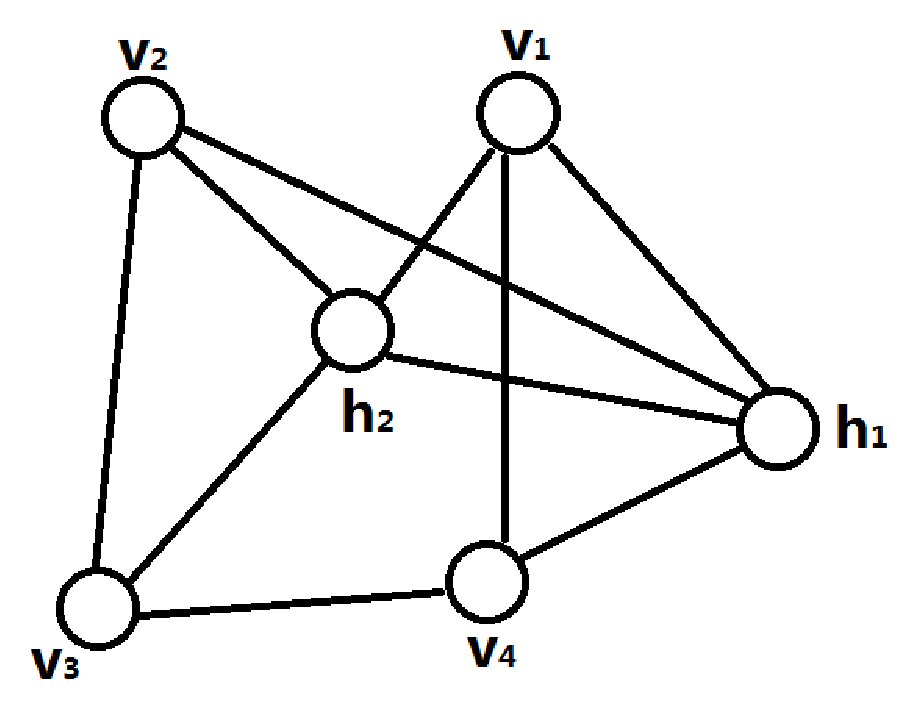
\includegraphics[width=0.3\textwidth]{BM1.eps}}}
\subfigure{\label{BM2}}\addtocounter{subfigure}{-2}
\subfigure{\subfigure[拓扑后的玻尔兹曼机]
			{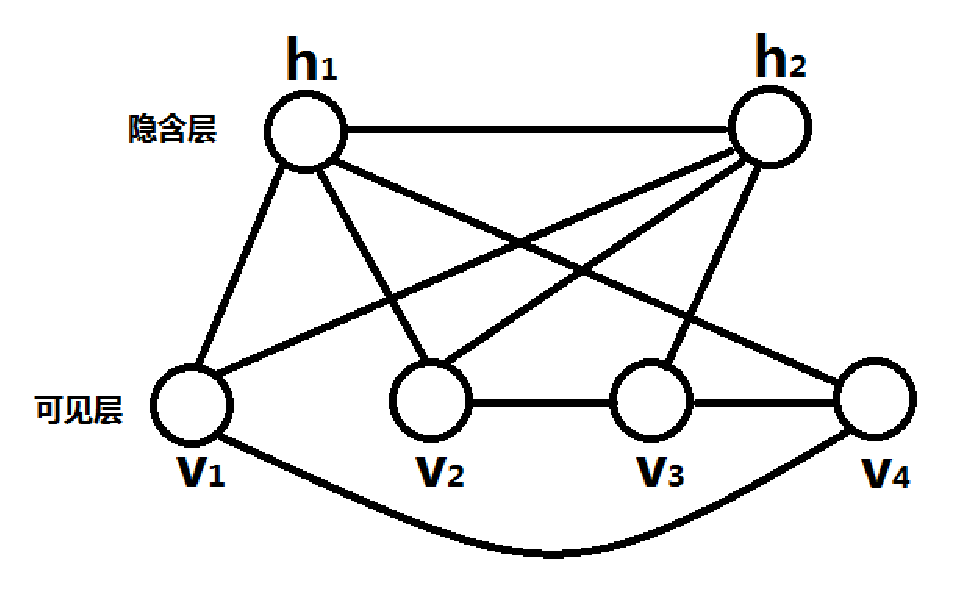
\includegraphics[width=0.4\textwidth]{BM2.eps}}}
\caption{玻尔兹曼机网络构型}
\label{img:BM}
\vspace{-1em}
\end{figure}

由图\ref{img:BM} 可见,在玻尔兹曼机中,可见节点与可见节点之间、隐含节点与隐含节点之间是可以有连接的,因此这是一个反馈网络。层内节点有连接可以大大地增强网络的表达能力,但是也大大地增加了网络的训练难度,因此玻尔兹曼机并没有非常成功地解决人工智能的任务。

\BiSection{受限玻尔兹曼机}
x在受限玻尔兹曼机(Restrict  Boltzmann Machine,RBM)中,我们取消层间连接,从而出发后经过若干次“移动”也无法回到原点,因此RBM也可以认为是一个有向无环图。其网络结构图\ref{img:RBM} 所示。

\begin{figure}[!htbp]
\centering
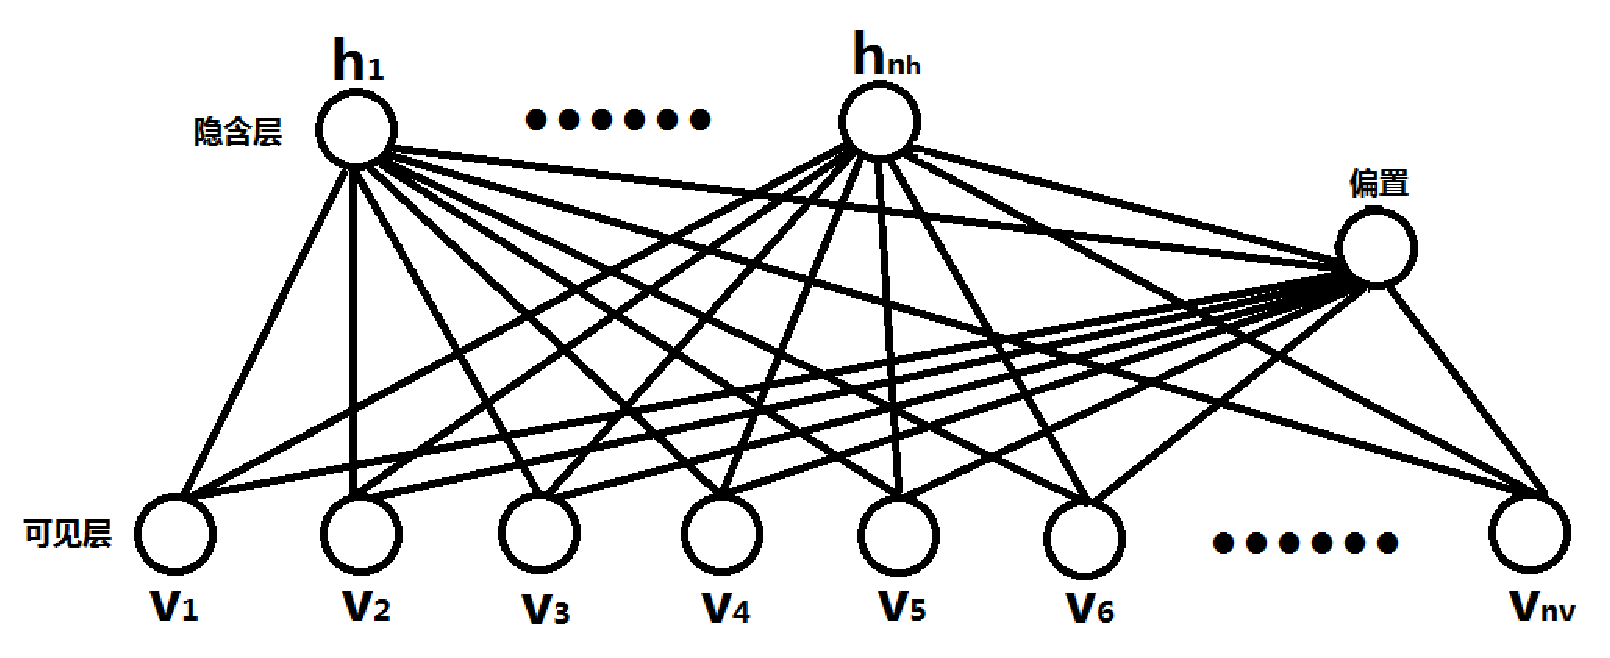
\includegraphics[width=0.7\textwidth]{RBM.eps}
\caption{RBM网络构型}
\label{img:RBM}
\end{figure}

为了方便往后的讨论,我们约定网络参数的数学符号如下

\begin{equation}
W_{n_h \times n_v } = \left[               %左括号
\begin{array}{cccc}  
w_{1,1} & w_{1,2} &\cdots & w_{1, n_v}\\  
w_{2,1} & w_{2,2} &\cdots & w_{2, n_v}\\
\vdots  & \vdots & \ddots  & \vdots\\
w_{n_h, 1} & w_{n_h, 2} & \cdots & w_{n_h, n_v}
\end{array}
\right]~~~~%%%%%%%%%%%%%%%%%%%%
v = \left[   
\begin{array}{cccc}  
v_1\\  
v_2\\
\vdots\\
v_{n_v}
\end{array}
\right]~~~~%%%%%%%%%%%%%%%%%%%
h = \left[   
\begin{array}{cccc}  
h_1\\  
h_2\\
\vdots\\
h_{n_h}
\end{array}
\right]~~~~%%%%%%%%%%%%%%%%
b_v = \left[   
\begin{array}{cccc}  
b_{v_1}\\  
b_{v_2}\\
\vdots\\
b_{v_{n_v}}
\end{array}
\right]~~~~%%%%%%%%%%%%%%%%%%%%%% 
b_h = \left[   
\begin{array}{cccc}  
b_{h_1}\\  
b_{h_2}\\
\vdots\\
b_{h_{n_h}}
\end{array}
\right]
\end{equation}
式中,$W_{n_h \times n_v }$代表网络的权值参数,$w_{ij}$代表第$i$个隐含节点到第$j$个可见节点间的连接权值,因此$W_{n_h \times n_v }$的第$i$行代表了通向$h_i$的所有连接的权值, 第$j$列代表了通往$v_j$的所有连接的权值。 $v$代表可见节点的状态,$h$代表隐含节点的状态,$b_v$代表隐含层到可见层的偏置,$b_h$代表可见层到隐含层的偏置。

在RBM中,我们定义其Lyapunov函数如下\citeup{energyBased}:
\begin{equation}\label{eq:RBMenergy}
E(v, h) = - \sum\limits_{i=1}^{n_v}b_{v_i}v_i - \sum\limits_{j=1}^{n_h}b_{h_j}h_j -  \sum\limits_{i=1}^{n_v} \sum\limits_{j=1}^{n_h} h_j w_{j, i}v_i
\end{equation}
若将\eqref{eq:RBMenergy}写成矩阵形式,则为:
\begin{equation}
E(v, h) = -b_v^T v - b_h^T h - h^T W v
\end{equation}
由正则分布的定义\eqref{zhengzefenbu},我们可以得到$v$,$h$的联合分布为
\begin{equation}\label{lian he fen bu}
p(v, h) = \frac{1}{Z} e^{-E(v, h)}
\end{equation}
其中配分函数$Z$为
\begin{equation}\label{partionFunc}
Z = \sum\limits_{v, h}e^{-E(v, h)}
\end{equation}
由于实际中我们往往只能观察到可见节点,因此对联合分布\eqref{lian he fen bu}边缘化得
\begin{equation}\label{p_x1}
p(v) = \sum\limits_h \frac{1}{Z}e^{-E(v, h)} = \frac{1}{Z}\sum\limits_h e^{-E(v, h)}
\end{equation}
这个$ p(v) $总可以写成如下形式:
\begin{equation}\label{p_x2}
p(v) = \frac{e^{-F(v)}}{Z}
\end{equation}
式中,我们称$ F(v)  $为自由能函数\citeup{learnForAI},由式\eqref{p_x1}与\eqref{p_x2},我们不难推出$ F(v)  $为
\begin{equation}\label{freeEnergyDef}
F(v) = -\ln\sum\limits_h e^{-E(v, h)}
\end{equation}

为了继续我们往下的讨论,我们不加证明地引入关于受限玻尔兹曼机的一个定理:
\begin{theorem}\label{theo:iid}
在RBM中,在给定可见元状态时,隐含元的激活条件独立;反之,在给定隐含元状态时,可见元的激活条件独立。
\end{theorem}

此外,我们还需引入一些记号
\begin{equation}
h_{-k} = (h_1, h_2, \cdots, h_{k-1}, h_{k+1},\cdots, h_{n_h})^T
\end{equation}
\begin{equation}
\alpha(k) = b_{h_k} + \sum\limits_{i=1}^{n_v} w_{k, i}v_i
\end{equation}
\begin{equation}
\beta(v, h_{-k}) = \sum\limits_{i=1}^{n_v} b_{v_i}v_i + \sum_{\substack{j=1\\ j\neq k}}^{n_h} b_{h_j}h_j +  \sum\limits_{i=1}^{n_v}  \sum_{\substack{j=1\\ j\neq k}}^{n_h} h_j w_{j, i}v_i
\end{equation}
即$h_{-k}$代表除$k$外的所有隐含元状态,$\beta(v, h_{-k})$代表除$h_k$外所有节点构成的能量函数。因此,总的能量函数\eqref{eq:RBMenergy}可以写为
\begin{equation}
E(v, h) = -\beta(v, h_{-k}) - h_k \alpha(k)
\end{equation}

下面我们来推导隐含层的激活函数,在给定可见节点状态时,对于节点$h_k$,其激活概率为
\begin{equation}\label{equ:prob}
P(h_k = 1| v)
\end{equation}
由定理\ref{theo:iid},式\eqref{equ:prob}等价于
\begin{equation}
\begin{split}
P(h_k = 1|h_{-k}, v) &= \frac{P(h_k = 1, h_{-k}, v)}{P(h_{-k}, v)}\\
&= \frac{P(h_k = 1, h_{-k}, v)}{P(h_k=0,h_{-k} , v) +P(h_k=1, h_{-k} , v)  }\\
&=\frac{1}{1 + \exp\Big(-E(h_k = 0, h_{-k}, v) +E(h_k = 1, h_{-k}, v)  \Big)}\\
&= \frac{1}{1 + \exp\Big[  \Big(\beta(v, h_{-k})+ \alpha(k)\cdot 0\Big) + \Big(-\beta(v, h_{-k})- \alpha(k)\cdot 1\Big)  \Big]}\\
&= \frac{1}{1 + e^{-\alpha(k)}}\\
&=sigmoid\Big(\alpha(k)\Big)
\end{split}
\end{equation}
因此,给定可见层状态时,隐含元$k$的激活概率为
\begin{equation}\label{p(h_k|v)}
P(h_k =1| v) = sigmoid(b_{h_k} + \sum\limits_{j=1}^{n_v}w_{k, j}v_j)
\end{equation}
同理可推导在给定隐含层状态时,可见元$k$的激活概率为
\begin{equation}\label{p(v_k|h)}
P(v_k = 1|h) = sigmoid(b_{v_k} + \sum\limits_{i=1}^{n_k}w_{i, k}h_i)
\end{equation}
由定理\ref{theo:iid}的独立性可知
\begin{equation}\label{p(h|v)}
P(h|v) = \prod\limits_{j=1}^{n_k}P(h_j|v)
\end{equation}
\begin{equation}\label{p(v|h)}
P(v|h) = \prod\limits_{i=1}^{n_v}P(v_i|h)
\end{equation}

在RBM中,我们的目标是训练参数$W$,$b_v$,$b_h$使得模型能成功地刻画出数据分布。为了方便起见,我们记$\theta = (W, b_v, b_h)$,注意,这并不是矩阵合并,而是将所有的参数用$\theta$来代替。

假定我们有一个训练集$S$
\begin{equation}
S = \{v^{(1)}, v^{(2)}, \cdots v^{(i)}, \cdots, v^{(n_s)}\}
\end{equation}
其中$n_s$为训练样本数,$v^{(i)}$为第$i$个样本且
\begin{equation}
v^{(i)} = [v_1^{(i)}, v_2^{(i)}, \cdots, v_{n_v}^{(i)} ]^T
\end{equation}

由于样本是独立的,因此似然函数为
\begin{equation}
\mathcal{L}(\theta) = \prod\limits_{i=1}^{n_s}P(v^{(i)})
\end{equation}
对应的对数似然为
\begin{equation}
\ell(\theta) = \ln \prod\limits_{i=1}^{n_s}P(v^{(i)}) = \sum\limits_{i=1}^{n_s} \ln P(v^{(i)}) 
\end{equation}

对于整个训练集,我们要优化参数,使得似然最大化,假设我们使用梯度上升方法,则针对某个样本$\hat{v}$ ,参数的更新规则为
\begin{equation}
\theta = \theta + \eta \frac{\partial\ln\mathcal{L}_{\hat{v}} }{\partial\theta}
\end{equation}
其中
\begin{equation}
\begin{split}
\ln\mathcal{L}_{\hat{v}} & = \ln P(\hat{v})\\
&=\ln\Big[\frac{1}{Z} \sum\limits_h e^{-	E(\hat{v}, h)}\Big] \\
&= \ln\sum\limits_h e^{-	E(\hat{v}, h)} - \ln Z\\
%&= \ln\sum\limits_h e^{-	E(\hat{v}, h)} - \ln\sum\limits_{v, h} e^{-	E(v, h)}
\end{split}
\end{equation}
从而
\begin{equation}
\begin{split}
 \frac{\partial\ln\mathcal{L}_{\hat{v}} }{\partial\theta} 
 &=  \frac{\partial}{\partial\theta}\Big[ \ln\sum\limits_h e^{-	E(\hat{v}, h)} \Big] - 
 %\frac{\partial}{\partial\theta}\Big[ \ln\sum\limits_{v, h} e^{-E(v, h)}  \Big]
 \frac{\partial}{\partial\theta}\ln Z
 \end{split}
\end{equation}
由式\eqref{partionFunc}、式\eqref{p_x1}、式\eqref{p_x2},得
\begin{equation}\label{temp1}
\begin{split}
 \frac{\partial\ln\mathcal{L}_{\hat{v}} }{\partial\theta} 
 &=  - \frac{\partial}{\partial\theta}F(\hat{v}) + \frac{1}{Z} \sum\limits_{v}e^{-F(v)}  \frac{\partial}{\partial\theta}F(v) \\
 &=  - \frac{\partial}{\partial\theta}F(\hat{v}) + \sum\limits_{v} p(v) \frac{\partial}{\partial\theta}F(v)
 \end{split}
\end{equation}
\iffalse
等号两边取期望,则对于某个特定的样本$\hat{v}$,其对数似然的期望梯度为
\begin{equation}
E_{\hat{v}}\bigg[  \frac{\partial\ln\mathcal{L}_{\hat{v}} }{\partial\theta} \bigg]
=  - E_{\hat{v}} \bigg[ \frac{\partial}{\partial\theta}F(\hat{v}) \bigg] + 
E_{v}\bigg[ \sum\limits_{v}\frac{\partial}{\partial\theta}F(v)\bigg]
\end{equation}
式中,$E_{\hat{v}}$代表某个样本的期望,$E_{v}$代表真实模型的期望。
\fi
通过自由能函数$F(v)$对参数$\theta$求偏导,我们有
\begin{equation}
\begin{split}
\frac{\partial}{\partial\theta}F(v)
&= \frac{\sum_h e^{-E(v, h)} \cdot \frac{\partial E(v, h)}{\partial \theta}}
{\sum_h e^{-E(v, h)}}\\
&= \sum\limits_h \frac{ e^{-E(v, h)}/Z }{\sum_h e^{-E(v, h)}/Z}\cdot
\frac{\partial E(v, h)}{\partial \theta} \\
&= \sum\limits_h \frac{p(v, h)}{p(v)}\cdot
\frac{\partial E(v, h)}{\partial \theta}
\end{split}
\end{equation}
从而,式\eqref{temp1}等价于
\begin{equation}\label{expectFunc}
\begin{split}
 \frac{\partial\ln\mathcal{L}_{\hat{v}} }{\partial\theta} 
 &=  - \sum\limits_h \frac{p(\hat{v}, h)}{p(\hat{v})} \cdot \frac{\partial E(\hat{v}, h)}{\partial \theta}+ \sum\limits_{v} p(v) \sum\limits_h \frac{p(v, h)}{p(v)}\cdot \frac{\partial E(v, h)}{\partial \theta}\\
 &=  - \sum\limits_h p(h|\hat{v})\cdot \frac{\partial E(\hat{v}, h)}{\partial \theta}
 + \sum\limits_{v, h}p(v, h)\frac{\partial E(v, h)}{\partial \theta}\\
 &= -\mathbb{E}_{p(h|\hat{v})}\bigg[ \frac{\partial E(\hat{v}, h)}{\partial \theta} \bigg]
 + \mathbb{E}_{p(v, h)}\bigg[\frac{\partial E(v, h)}{\partial \theta}\bigg]
 \end{split}
\end{equation}
式中,$\mathbb{E}_{p(h|\hat{v})}$为$p(h|\hat{v})$分布下的期望,$\mathbb{E}_{p(v, h)}$为$p(v, h)$分布下的期望。

通过式\eqref{expectFunc},我们就可以计算相对于某个样本$\hat{v}$的对数似然梯度。式\eqref{expectFunc}中的第一项是容易计算的,因为我们已经推导出了$p(h|v)$的分布形式,即式\eqref{p(h_k|v)}和式\eqref{p(h|v)}。由于我们简记$\theta = (W, b_v, b_h)$,因此我们需要对$W$,$ b_v $,$ b_h $三个参数分别推导梯度公式。
\begin{equation}\label{deltaW}
\begin{split}
\sum\limits_h p(h|v)\frac{\partial E(v, h)}{\partial w_{ij}}
=&-\sum\limits_h \prod\limits_{k=1}^{n_h} p(h_k|v) h_i v_j \\
=&-\sum\limits_{h_i} \sum\limits_{h_{-i}} p(h_i|v)p(h_{-i}|v)h_i v_j \\
=& -\sum\limits_{h_i}  p(h_i|v)h_i v_j \sum\limits_{h_{-i}}p(h_{-i}|v) \\
=& -\sum\limits_{h_i}  p(h_i|v)h_i v_j \\
=& -\sum\limits_{h_i}  p(h_i|v)v_j
\end{split}
\end{equation}
\begin{equation}\label{deltaHidBais}
\begin{split}
\sum\limits_h p(h|v)\frac{\partial E(v, h)}{\partial b_{h_i}}
=&-\sum\limits_h \prod\limits_{k=1}^{n_h} p(h_k|v) h_i\\
=&-\sum\limits_{h_i} \sum\limits_{h_{-i}} p(h_i|v)p(h_{-i}|v)h_i\\
=& -\sum\limits_{h_i}  p(h_i|v)h_i\sum\limits_{h_{-i}}p(h_{-i}|v) \\
=& -\sum\limits_{h_i}  p(h_i|v)h_i\\
=& -\sum\limits_{h_i}  p(h_i|v)
\end{split}
\end{equation}
\begin{equation}\label{deltaVisBais}
\begin{split}
\sum\limits_h p(h|v)\frac{\partial E(v, h)}{\partial b_{vi}}
=& - \sum\limits_h p(h|v) v_i\\
=&- v_i
\end{split}
\end{equation}

尽管我们可以很容易地通过式\eqref{deltaW}、 式\eqref{deltaHidBais}、式\eqref{deltaVisBais}计算式\eqref{expectFunc}中的第一项,但是第二项却无法计算,因为第二项涉及到归一化因子$Z$,这将是$O(2^{n_v+n_h})$复杂度的项,因此我们需要使用马尔可夫链蒙特卡罗方法(MCMC)进行处理。

\BiSection{本章小结}
x本章中,我们从伊辛模型出发,引入玻尔兹曼机,进一步推广到受限波尔兹曼机。在受限玻尔兹曼机中,我们建立了对数据描述的概率分布即正则分布,随后,我们推导出受限玻尔兹曼机中由可见节点激活隐含节点以及由隐含节点激活可见节点所使用的公式,此时,如果整个网络的参数是确定的,那么,利用这个网络可以刻画数据的特征。但由于未经训练的网络参数是未知的,我们需要使用样本来求取参数的近似值,求取的方法我们使用极大似然,为了使用梯度下降方法最大化似然函数,我们对似然函数求导,进而得到每一步迭代所使用的梯度。但由于这个梯度有一项不容易求取,我们需要利用马尔可夫链蒙特卡罗方法来处理,但本章没有详细讨论,因此,本章节并不是一个独立的章节,考虑到马尔可夫链蒙特卡罗方法所蕴含的内容较多,所以我们将其独立成为一章。